\subsection{Geheugenbeheer in Windows}

De Windows virtual memory manager controleert hoe het geheugen toegewezen wordt en hoe de paginering gebeurd.

Het is ontwikkeld om te werken voor uiteenlopende platforms en ondersteunt paginagroottes van 4KB tot 64 KB.

\subsubsection{Weergave van virtuele adressen in Windows}

Elk gebruikersproces in Windows heeft een afzonderlijke 32-bit adresruimte, wat 4 GB geheugen per proces mogelijk maakt. Een gedeelte hiervan is gereserveerd voor het besturingssysteem.

Normaal gezien heeft ieder gebruikersproces 2 GB beschikbare virtuele adresruimte. (slides staat 32 GB maar da moet een fout zijn!). Alle gebruikersprocessen delen een 2 GB systeemruimte.


\begin{figure}[htp]
    \centering
            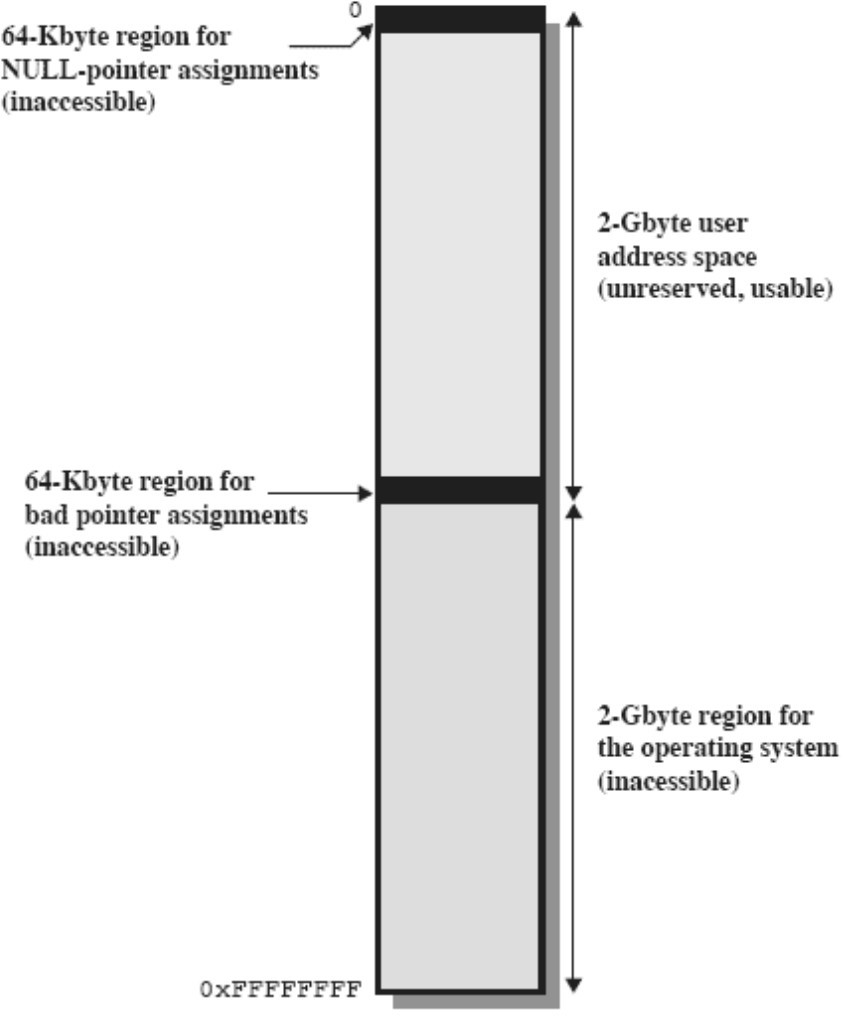
\includegraphics[width=4in]{img/weergavevirtueel}
        \caption{}
    \label{fig:}
\end{figure}


\subsubsection{Paginering in Windows}

Bij de creatie van een proces kan het proces gebruik maken van de volledige gebruikersruimte van 2 GB.

Deze ruimte is verdeeld in pagina’s met een vaste grootte toegewezen in regio’s van 64 KB. De regio’s kunnen zich in 3 toestanden bevinden:

\begin{itemize}
\item Beschikbaar
\item Gereserveerd
\item Toegewezen
\end{itemize}

Voor het beheer van de residente set gebruikt Windows een systeem met variabele toewijzing met lokaal bereik.

Wanneer een proces voor het eerst wordt geactiveerd, wordt daaraan een bepaald aantal paginaframes hoofdgeheugen toegewezen als werkset van dat proces.

Werksets van actieve processen worden aangepast aan de hoeveelheid beschikbare hoofdgeheugen.

Is er veel hoofdgeheugen, dan staat de VMM toe dat de residente sets van de actieve processen blijven groeien. Is er te weinig hoofdgeheugen, dan zal de VMM de minder recent gebruikte pagina’s verwijderen uit de werkset van actieve processen.




